\subsection{Pojęcia i zasady}

\subsubsection{Wstęp}
Ten rozdział dokumentuje \hyperlink{def:lupus}{\textbf{Lupus}} w formie wyjaśniania zdefiniowanych na jego potrzeby pojęć, konceptów i zasad. Są one punktem wyjścia do dokładniejszych specyfikacji i zarazem zrozumienia architektury systemu. Rozdział ten zawiera wiele odnośników do definicji znajdujących się w załącznikach i nie wszystkie pojęcia tłumaczone są w tym rozdziale.

\subsubsection{Problem zarządzania}

W rzeczywistym świecie często napotkamy sytuacje, w których byłoby dobrze, gdyby praca jakiegoś systemu mogła być stale regulowana. Na przykład:

\begin{itemize}
    \item chcielibyśmy, aby samochody miały funkcję regulującą pracę silnika w celu utrzymania stałej prędkości,
    \item przydałoby się, gdyby lodówka mogła utrzymywać chłodną, ale nie ujemną temperaturę, niezależnie od tego, jak często otwierane są drzwi lub jaka jest temperatura na zewnątrz,
    \item byłoby korzystne, gdyby serwer w chmurze mógł zagwarantować, że aplikacja z wystarczającymi zasobami do pokrycia potrzeb użytkowników będzie uruchomiona i działała.
\end{itemize}

Problemy wymienione powyżej można traktować jako \hyperlink{def:problem-zarzadzania}{\textbf{problemy zarządzania}} (ang. \textit{management problems}). Nazwa bierze się stąd, że nie ma żadnych technicznych ograniczeń uniemożliwiających osiągnięcie tych celów. Wszystkie wymienione systemy są odpowiednio wyposażone; np. możemy dodać więcej paliwa do silnika lub dostarczyć więcej mocy do sprężarki w lodówce. Problem leży w faktycznym wykonaniu tych czynności w odpowiednich momentach np. dodanie więcej paliwa, gdy auto zwalnia lub dostarczenie większej mocy, gdy temperatura w lodówce wzrasta. Dlatego jest to problem czystego zarządzania.

Systemem, którym chcemy zarządzać, nazywamy \hyperlink{def:system-zarzadzany}{\textbf{System Zarządzany}} (ang. \textit{managed system}).

\subsubsection{System Sterowania}

\hyperlink{def:system-sterowania}{\textbf{System Sterowania}} (ang. \textit{Control System\footnote{innym tłumaczeniem na polski jest "regulator"}}) to system, który reguluje pracą \hyperlink{def:system-zarzadzany}{\textbf{Systemu Zarządzanego}}. Przykładowo jest to:
\begin{itemize}
    \item tempomat, który reguluje pracą silnika w celu utrzymania stałej prędkości,
    \item lodówka, która reguluje pracą sprężarki w celu utrzymania stałej, chłodnej temperatury,
    \item Kubernetes, który reguluje liczbę działających Podów, aby utrzymać pożądaną dostępność aplikacji.
\end{itemize}

Innymi słowy mówiąc, \hyperlink{def:system-sterowania}{\textbf{System Sterowania}} rozwiązuje \hyperlink{def:problem-zarzadzania}{\textbf{Problem Zarządzania}}.

\subsubsection{Pętla Sterowania}

Ogólną architekturą \hyperlink{def:system-sterowania}{\textbf{Systemów Sterowania}} używaną do rozwiązywania \hyperlink{def:problem-zarzadzania}{\textbf{Problemów Zarządzania}} jest \hyperlink{def:petla-sterowania}{\textbf{Pętla Sterowania}}.

Pętle sterowania są klasyfikowane w zależności od tego, czy wykorzystują mechanizmy sprzężenia zwrotnego (ang. \textit{feedback mechanism}):
\begin{itemize}
    \item \hyperlink{def:petla-sterowania}{\textbf{Otwarte Pętle Sterowania}}: \hyperlink{def:akcja-sterujaca}{\textbf{Akcja Sterująca}} (ang. \textit{Control Action}) (czyli wejście do \hyperlink{def:system-zarzadzany}{\textbf{Systemu Zarządzanego}}) jest niezależne od wyjścia \hyperlink{def:system-zarzadzany}{\textbf{Systemu Zarządzanego}}.
    \item \hyperlink{def:zamknieta-petla-sterowania}{\textbf{Zamknięte Pętle Sterowania}}: Wyjście \hyperlink{def:system-zarzadzany}{\textbf{Systemu Zarządzanego}} jest sprzężane do wejścia \hyperlink{def:system-sterowania}{\textbf{Systemu Sterowania}} i wpływa na \hyperlink{def:akcja-sterujaca}{\textbf{Akcję Sterującą}}. 
\end{itemize}

W \hyperlink{def:lupus}{\textbf{Lupus}} bierzemy pod uwagę wyłącznie \hyperlink{def:zamknieta-petla-sterowania}{\textbf{Zamknięte Pętle Sterowania}}.

\subsubsection{Zamknięta Pętla Sterowania}

Jest to punkt wyjściowy dla naszej architektury referencyjnej (rys. \ref{fig:33-arch}).

\begin{figure}[!h]
    \centering 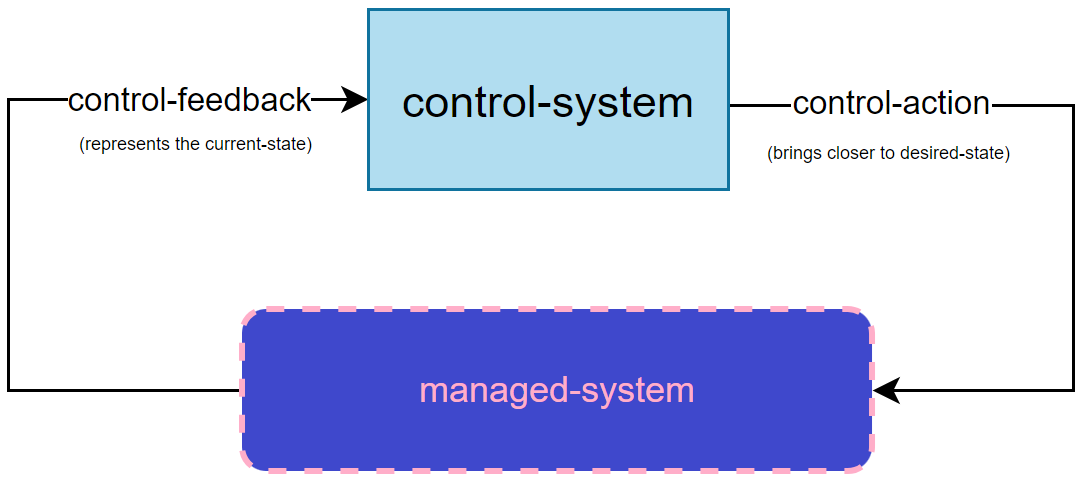
\includegraphics[width=1\linewidth]{33-arch.png}
    \caption{Architektura referencyjna dla Lupus. Źródło: Opracowanie własne.}\label{fig:33-arch}
\end{figure}

Architekturę (rys. \ref{fig:33-arch}) należy czytać, mając na uwadze następujące definicje:

\begin{itemize}
    \item \hyperlink{def:system-sterowania}{\textbf{System Sterowania}} (ang. \textit{Control System}) - system, który rozwiązuje \hyperlink{def:problem-zarzadzania}{\textbf{Problem Zarządzania}} występujący w \hyperlink{def:system-zarzadzany}{\textbf{Systemie Zarządzanym}} za pomocą \hyperlink{def:zamknieta-petla-sterowania}{\textbf{Zamkniętej Pętli Sterowania}}. W każdej iteracji \hyperlink{def:system-sterowania}{\textbf{System Sterowania}} analizuje \hyperlink{def:sprzezenie-zwrotne}{\textbf{Sprzężenie Zwrotne}} (ang. \textit{Control Feedback}) i \textit{wnioskuje} \hyperlink{def:akcja-sterujaca}{\textbf{Akcję Sterującą}}.
    \item \hyperlink{def:zamknieta-petla-sterowania}{\textbf{Zamknięta Pętla Sterowania}} - nieskończona pętla, która reguluje stan \hyperlink{def:system-zarzadzany}{\textbf{Systemu Zarządzanego}}, iteracyjnie zbliżając jego \hyperlink{def:stan-aktualny}{\textbf{Stan Aktualny}} do \hyperlink{def:stan-pozadany}{\textbf{Stanu Pożądanego}}. 
    \item \hyperlink{def:akcja-sterujaca}{\textbf{Akcja Sterująca}} (ang. \textit{Control Action}) - akcja wykonywana na \hyperlink{def:system-zarzadzany}{\textbf{Systemie Zarządzanym}}, która ma na celu przybliżenie go do \hyperlink{def:stan-pozadany}{\textbf{Stanu Pożądanego}}.
    \item \hyperlink{def:sprzezenie-zwrotne}{\textbf{Sprzężenie Zwrotne}} (ang. \textit{Control Feedback}) - reprezentacja \hyperlink{def:stan-aktualny}{\textbf{Stanu Aktualnego}} wysyłana z (odbierana od) \hyperlink{def:system-zarzadzany}{\textbf{Systemu Zarządzanego}}.
\end{itemize}

W powyższej architekturze \hyperlink{def:lupus}{\textbf{Lupus}} pełni rolę \hyperlink{def:system-sterowania}{\textbf{Systemu Sterowania}}.


\subsubsection{Agenci Translacyjni}
Z racji, że każdy system, bez żadnych modyfikacji (\hyperref[req:15]{Wymaganie 15}) może wejść w rolę \hyperlink{def:system-zarzadzany}{\textbf{Systemu Zarządzanego}}, potrzebujemy warstwy integracji między \hyperlink{def:system-zarzadzany}{\textbf{Systemem Zarządzanym}} a \hyperlink{def:lupus}{\textbf{Lupus}}, podobnej do koncepcji "API Broker" w architekturze \hyperlink{def:eni}{ENI} (rys. \ref{fig:23-eni-arch}). Tak narodziła się koncepcja \hyperlink{def:agent-translacji}{\textbf{Agentów Translacji}} (ang. \textit{Translation Agents}). 

W każdym \hyperlink{def:wdrozenie-lupus}{\textbf{wdrożeniu Lupus}}, \hyperlink{def:uzytkownik}{\textbf{Użytkownik}} musi stworzyć \hyperlink{def:agent-translacji}{\textbf{Agentów Translacyjnych}}. 

Z punktu widzenia komunikacji, każdego \hyperlink{def:agent-translacji}{\textbf{Agenta Translacyjnego}} możemy podzielić na dwie części:
\begin{itemize}
    \item Część komunikująca się z \hyperlink{def:system-zarzadzany}{\textbf{Systemem Zarządzanym}}. Jest zewnętrzna względem \hyperlink{def:lupus}{\textbf{Lupus}} i nie podlega żadnej specyfikacji.
    \item Część komunikująca się z \hyperlink{def:lupus}{\textbf{Lupus}}. Musi być zgodna z jednym z \hyperlink{def:interfejsy-lupus}{\textbf{Interfejsów Lupus}}: \hyperlink{def:interfejs-lupin}{\textbf{Lupin}} lub \hyperlink{def:interfejs-lupout}{\textbf{Lupout}}.
\end{itemize}

Mamy dwóch \hyperlink{def:agent-translacji}{\textbf{Agentów Translacji}}, jednego do komunikacji przychodzącej (ang. \textit{Ingress}) i jednego do wychodzącej (ang. \textit{Egress}). 

W każdej iteracji pętli zadaniem \hyperlink{def:agent-ingress}{\textbf{Agenta Ingress}} jest odbieranie/zbieranie \hyperlink{def:sprzezenie-zwrotne}{\textbf{Sprzężenia Zwrotnego}} z \hyperlink{def:system-zarzadzany}{\textbf{Systemu Zarządzanego}} i translacja go na format zrozumiały przez \hyperlink{def:lupus}{\textbf{Lupus}} za pomocą \hyperlink{def:interfejs-lupin}{\textbf{Interfejsu Lupin}}. Z kolei zadaniem \hyperlink{def:agent-egress}{\textbf{Agenta Egress}} jest odbieranie \hyperlink{def:finalne-dane}{\textbf{Finalnych Danych}} i translacja ich na \hyperlink{def:akcja-sterujaca}{\textbf{Akcję Sterującą}}, która później zostaje wysłana do (lub przeprowadzona na) \hyperlink{def:system-zarzadzany}{\textbf{Systemie Zarządzanym}}.

Architektura wraz z wprowadzeniem \hyperlink{def:agent-translacji}{\textbf{Agentów Translacji}} ukazana jest na rysunku \ref{fig:33-arch2}.

\begin{figure}[!h]
    \centering 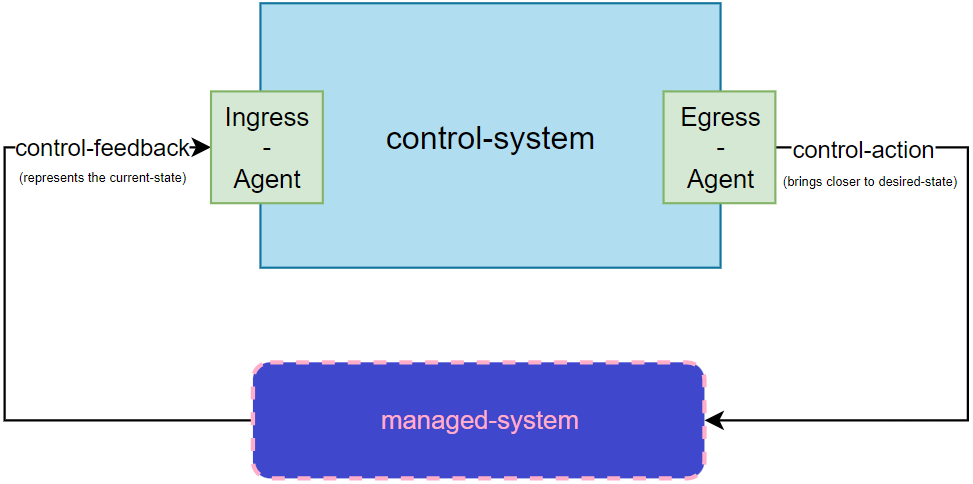
\includegraphics[width=1\linewidth]{33-arch2.png}
    \caption{Architektura referencyjna z agentami translacji. Źródło: Opracowanie własne.}\label{fig:33-arch2}
\end{figure}

Specyfikacja interfejsów \hyperlink{def:interfejs-lupin}{\textbf{Lupin}} oraz \hyperlink{def:interfejs-lupout}{\textbf{Lupout}} zawarta jest w \hyperref[appendix:4]{Załączniku 4}.

\subsubsection{Workflow pętli}

Kiedy \hyperlink{def:lupus}{\textbf{Lupus}} otrzyma \hyperlink{def:stan-aktualny}{\textbf{Stan Aktualny}} poprzez interfejs \hyperlink{def:interfejs-lupin}{\textbf{Lupin}}, rozpoczyna się \hyperlink{def:workflow-petli}{\textbf{Workflow Pętli}}, które ma na celu dostarczać \hyperlink{def:logika-petli}{\textbf{Logikę Pętli}} (ang. \textit{Loop Logic}) i składa się z \hyperlink{def:element-petli}{\textbf{Elementów Pętli}} (ang. \textit{Loop Elements}). 

Elementem pętli może być zarówno:
\begin{itemize}
    \item \hyperlink{def:element-lupus}{\textbf{Element Lupus}}, który działa w warstwie sterowania Kubernetes, a jego misją jest wykonywać \hyperlink{def:workflow-petli}{\textbf{Workflow Pętli}}.
    \item referencja do \hyperlink{def:element-zewnetrzny}{\textbf{Elementu Zewnętrznego}}, który działa poza warstwą sterowania Kubernetes, a jego misją jest wykonywać \hyperlink{def:czesc-obliczeniowa}{\textbf{Część Obliczeniową}} \hyperlink{def:logika-petli}{\textbf{Logiki Pętli}}.
\end{itemize}

\hyperlink{def:workflow-petli}{\textbf{Workflow Pętli}} jest wyrażany w \hyperlink{def:lupn}{\textbf{LupN}}, specjalnej notacji do opisywania workflow pętli, której dokładna specyfikacja znajduje się w \hyperref[appendix:3]{Załączniku 3}.

Przykładowe \hyperlink{def:workflow-petli}{\textbf{Workflow Pętli}} pokazano na rysunku \ref{fig:33-workflow}.

\begin{figure}[!h]
    \centering 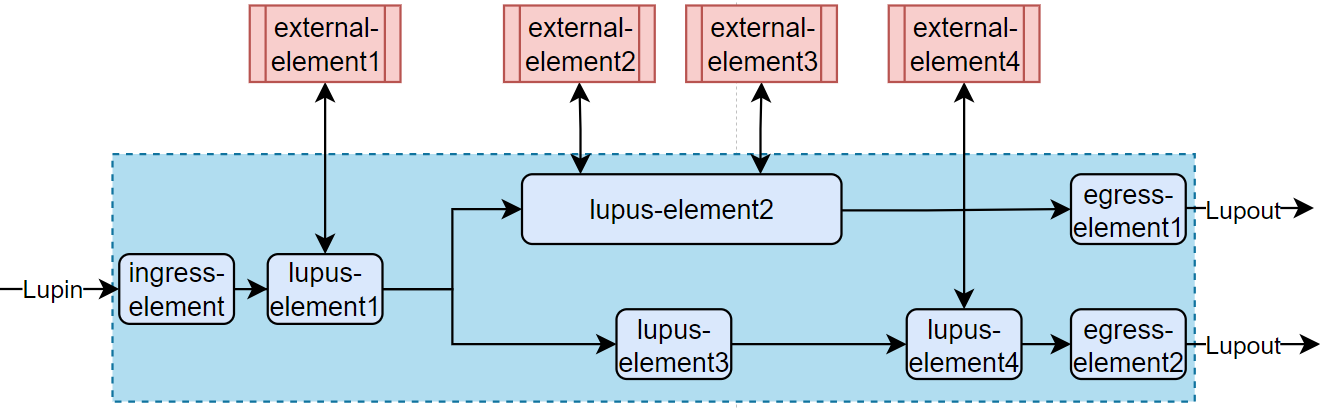
\includegraphics[width=1\linewidth]{33-workflow.png}
    \caption{Przykładowe workflow pętli. Źródło: Opracowanie własne.}\label{fig:33-workflow}
\end{figure}

\begin{itemize}
    \item Niebieskie, zaokrąglone prostokąty reprezentują \hyperlink{def:element-lupus}{\textbf{Elementy Lupus}}.
    \item Czerwone prostokąty oznaczają \hyperlink{def:element-zewnetrzny}{\textbf{Elementy Zewnętrzne}}.
    \item Niebieski obszar wyznaczony linią przerywaną wskazuje elementy działające w warstwie sterowania Kubernetes. 
    \item Wyróżniono \hyperlink{def:element-lupus}{\textbf{Elementy Lupus}} odpowiedzialne za \hyperlink{def:interfejs-lupin}{\textbf{Ingress}} i \hyperlink{def:interfejs-lupout}{\textbf{Egress}}.
\end{itemize}

\hyperlink{def:element-zewnetrzny}{\textbf{Elementy Zewnętrzne}} to zazwyczaj serwery HTTP (w szczególności serwery \hyperlink{def:opa}{\textbf{Open Policy Agent}}).

Jeden \hyperlink{def:element-lupus}{\textbf{Element Lupus}} może komunikować się z żadnym, jednym lub wieloma \hyperlink{def:element-zewnetrzny}{\textbf{Elementami Zewnętrznymi}}, a liczba ta może się różnić w każdej iteracji pętli.

\subsubsection{Dane i Akcje}

\hyperlink{def:dane}{\textbf{Dane}} (ang. \textit{data}) to nośnik informacji w ramach jednej iteracji pętli w formacie JSON. Na wejściu \hyperlink{def:element-ingres}{\textbf{Elementu Ingress}} reprezentują one \hyperlink{def:stan-aktualny}{\textbf{Stan Aktualny}} \hyperlink{def:system-zarzadzany}{\textbf{Systemu Zarządzanego}}. Następnie, w trakcie iteracji pętli, \hyperlink{def:projektant}{\textbf{Projektant}} decyduje, jakie informacje będą przenosić. Zazwyczaj są to informacje związane z \hyperlink{def:logika-petli}{\textbf{Logiką Pętli}}, takie jak wejścia (ang. \textit{inputs}) do \hyperlink{def:element-zewnetrzny}{\textbf{Elementów Zewnętrznych}} oraz ich odpowiedzi. Na końcu iteracji, gdy \hyperlink{def:dane}{\textbf{Dane}} trafiają do \hyperlink{def:agent-egress}{\textbf{Agenta Egress}}, muszą reprezentować \hyperlink{def:akcja-sterujaca}{\textbf{Akcję Sterowania}}. 

Działanie pojedynczego \hyperlink{def:element-lupus}{\textbf{Elementu Lupus}} jest opisane poprzez \hyperlink{def:workflow-petli}{\textbf{Workflow Akcji}}. \hyperlink{def:akcja}{\textbf{Akcje}} wykonują różne operacje na \hyperlink{def:dane}{\textbf{Danych}}. Istnieje wiele rodzajów akcji, a kluczowym typem akcji jest "Send", która pozwala komunikować się \hyperlink{def:element-lupus}{\textbf{Elementowi Lupus}} z \hyperlink{def:element-zewnetrzny}{\textbf{Elementem Zewnętrznym}}. Inne typy akcji służą organizacji danych.

\begin{figure}[!h]
    \centering 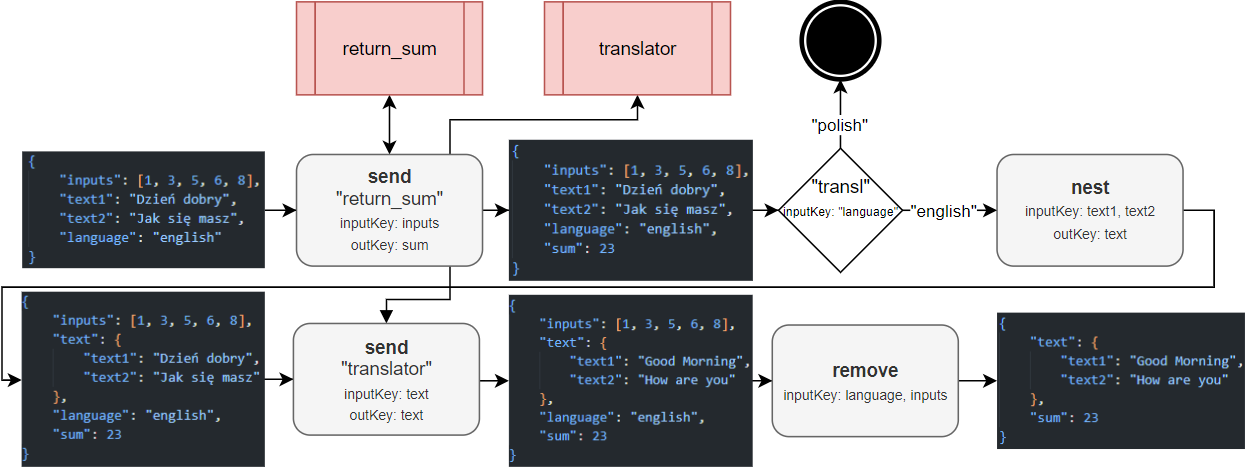
\includegraphics[width=1\linewidth]{33-workflow-akcji.png}
    \caption{Przykładowe workflow akcji. Źródło: Opracowanie własne.}\label{fig:33-workflow-akcji}
\end{figure}

Pełna specyfikacja \hyperlink{def:dane}{\textbf{Danych}} znajduje się w \hyperref[appendix:5]{Załączniku 5}, zaś pełna specyfikacja \hyperlink{def:akcja}{\textbf{Akcji}} w \hyperref[appendix:6]{Załączniku 6}.

\subsubsection{Open Policy Agent}

\hyperlink{def:opa}{\textbf{Open Policy Agent}} (OPA) to otwartoźródłowe narzędzie przeznaczone do definiowania, egzekwowania i zarządzania politykami w systemach oprogramowania. Systemy informatyczne odpytują serwery \hyperlink{def:opa}{\textbf{OPA}} podczas wykonywania operacji, które wymagają decyzji (np. decyzji dostępu, konfiguracji czy zachowania aplikacji). Dzięki takiemu podejściu można oddzielić logikę podejmowania decyzji od kodu aplikacji, co zwiększa modularność, wprowadza centralny punkt zarządzania politykami oraz ułatwia utrzymanie systemów.

Polityki w \hyperlink{def:opa}{\textbf{OPA}} definiowane są w języku Rego. Jest to deklaratywny język stworzony specjalnie na potrzeby \hyperlink{def:opa}{\textbf{OPA}}. Pozwala na tworzenie złożonych reguł i logiki decyzji. Oficjalna strona projektu dostępna jest pod linkiem: \url{https://www.openpolicyagent.org}.

\begin{lstlisting}[language=sh, caption={\emph{Przykładowy kod rego}}\label{lst:1}]
allow {
    input.user.role == "admin"
}

allow {
    input.user.role == "user"
    input.action == "read"
}
\end{lstlisting}

\hyperlink{def:opa}{\textbf{Open Policy Agent}} jest rekomendowanym \hyperlink{def:element-zewnetrzny}{\textbf{Elementem Zewnętrznym}} dla \hyperlink{def:lupus}{\textbf{Lupus}}.